% Página
\section{Autenticidade}

A Autenticidade está relacionada à verificação da identidade das partes envolvidas na comunicação e à garantia de que a origem das informações é confiável. Este pilar garante que as entidades (pessoas, sistemas ou dispositivos) sejam quem dizem ser e que as informações provenientes dessas entidades sejam genuínas. Métodos de autenticação, como senhas, certificados digitais e autenticação de dois fatores, são utilizados para validar a identidade e estabelecer a confiança entre as partes. A autenticidade é crucial para prevenir fraudes e assegurar a legitimidade das transações eletrônicas.

\subsection{Assinatura Digital}

Uma assinatura digital permite verificar se uma mensagem corresponde a uma assinatura produzida com a chave privada associada à chave pública usada na verificação. Ela ajuda a detectar alterações na mensagem e a autenticar a origem da assinatura, desde que a chave pública esteja autenticada. A assinatura digital não cifra a mensagem nem fornece confidencialidade.\\

\textbf{Funcionamento}\\

Bob calcula uma assinatura \(\sigma=\mathrm{Sign}(KPrBob,T)\) sobre a mensagem \(T\) e envia a mensagem junto com \(\sigma\). Na prática, algoritmos de assinatura costumam aplicar internamente uma função de hash; isso não significa que o resumo seja simplesmente cifrado com a chave privada. Alice verifica a assinatura com \(\mathrm{Verify}(KPuBob,T,\sigma)\), que retorna válida ou inválida.

A Figura \ref{fig:assinatura} mostra esse fluxo. Alice precisa obter uma chave pública que esteja de fato associada a Bob, por exemplo validando a cadeia de certificados ou conferindo o fingerprint por um canal independente. Sem essa validação, um atacante poderia substituir a chave pública por outra e fazer Alice aceitar uma assinatura sob a chave errada. Uma verificação válida confirma a correspondência entre mensagem, assinatura e chave pública; a atribuição da identidade de Bob depende da confiança nessa chave.

\begin{figure}[H]
	\centering
	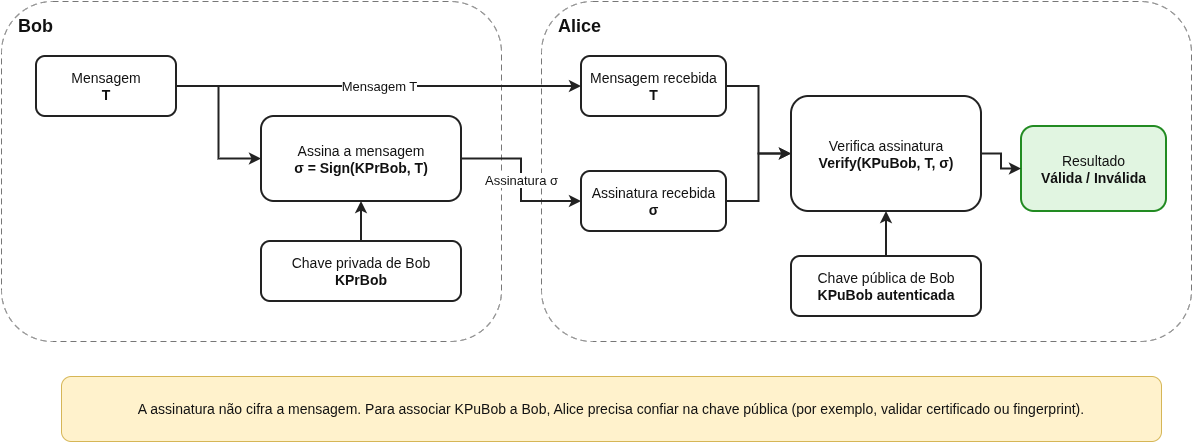
\includegraphics[scale=0.40]{assinatura.png}
	\caption{Bob assina uma mensagem e Alice verifica a assinatura com a chave pública autenticada}
	\label{fig:assinatura}
\end{figure}

\begin{enumerate}
	\item \textbf{Criação do par de chaves:}
	Bob gera uma chave privada RSA e extrai dela a chave pública correspondente. A chave privada deve permanecer sob o controle de Bob; a chave pública deve ser autenticada antes de Alice confiar nela.
	\begin{tcolorbox}[width=\textwidth]
	{\small
		\begin{verbatim}
		$ umask 077
		$ openssl genpkey -algorithm RSA -out KPrBob.pem -pkeyopt rsa_keygen_bits:3072
		$ openssl pkey -in KPrBob.pem -pubout -out KPuBob.pem
		\end{verbatim}
	}
	\end{tcolorbox}

	\item \textbf{Assinatura da mensagem:}
	Bob assina os bytes de \texttt{arquivo.txt} com RSA-PSS e SHA-256. Ele envia o arquivo original e \texttt{signature.bin} para Alice.
	\begin{tcolorbox}[width=\textwidth]
	{\small
		\begin{verbatim}
		$ openssl dgst -sha256 -sign KPrBob.pem \
		  -sigopt rsa_padding_mode:pss \
		  -sigopt rsa_pss_saltlen:digest \
		  -out signature.bin arquivo.txt
		\end{verbatim}
	}
	\end{tcolorbox}

	\item \textbf{Verificação da assinatura:}
	Alice verifica a assinatura sobre a cópia recebida de \texttt{arquivo.txt}, usando a chave pública autenticada de Bob e os mesmos parâmetros RSA-PSS.
	\begin{tcolorbox}[width=\textwidth]
	{\small
		\begin{verbatim}
		$ openssl dgst -sha256 -verify KPuBob.pem \
		  -sigopt rsa_padding_mode:pss \
		  -sigopt rsa_pss_saltlen:digest \
		  -signature signature.bin arquivo.txt
		Verified OK
		\end{verbatim}
	}
	\end{tcolorbox}
	Uma verificação bem-sucedida indica que a assinatura corresponde ao arquivo e à chave pública fornecidos. Se a mensagem ou a assinatura tiver sido alterada, ou se for usada outra chave pública, a verificação falha.
\end{enumerate}

\textbf{O que a assinatura garante}

\begin{itemize}
	\item \textbf{Integridade:} permite detectar alterações nos dados assinados.
	\item \textbf{Autenticidade da chave:} confirma que a assinatura corresponde à chave privada associada à chave pública usada; associar essa chave a Bob exige autenticar a chave pública.
	\item \textbf{Sem confidencialidade:} qualquer pessoa que obtenha a mensagem pode lê-la; para ocultar seu conteúdo, é necessário cifrá-la separadamente.
\end{itemize}

\pagebreak
